\documentclass[11pt]{article}
\usepackage[T1]{fontenc}
\usepackage{lmodern,microtype}
\usepackage[margin=1in]{geometry}
\usepackage{amsmath,amssymb,amsthm,mathtools}
\usepackage{booktabs,longtable,array,enumitem}
\usepackage{xcolor,tikz}
\usetikzlibrary{arrows.meta,positioning}
\usepackage[colorlinks=true,linkcolor=blue!45!black,citecolor=blue!45!black,urlcolor=blue!45!black]{hyperref}
\usepackage{xurl}
\usepackage{fancyhdr}
\pagestyle{fancy}\fancyhf{}\fancyhead[L]{\small Four-copy kernels for boundary patterns}\fancyhead[R]{\small ProveIt research continuation}\fancyfoot[C]{\thepage}
\setlength{\headheight}{14pt}
\newtheorem{theorem}{Theorem}[section]
\newtheorem{lemma}[theorem]{Lemma}
\newtheorem{proposition}[theorem]{Proposition}
\newtheorem{corollary}[theorem]{Corollary}
\newtheorem{definition}[theorem]{Definition}
\theoremstyle{remark}\newtheorem{remark}[theorem]{Remark}
\newcommand{\FF}{\mathcal F}
\newcommand{\Sig}{\mathsf S}
\newcommand{\cut}{\delta}
\newcommand{\cl}{\operatorname{cl}}
\newcommand{\bits}{\operatorname{bits}}
\newcommand{\poly}{\operatorname{poly}}
\DeclareRobustCommand{\code}[1]{\nolinkurl{#1}}
\newcommand{\infk}{\infty_k}
\DeclareMathOperator{\lcm}{lcm}
\title{\textbf{Four-Copy Kernels for Compressed Boundary Patterns}\\[0.5em]
\large Marked cut signatures, sharp repetition bounds, and certified terminal tests for unknot hierarchies}
\author{Research continuation for the ProveIt project\\\small Prepared with ChatGPT; proofs and implementation supplied for review}
\date{12 October 2026}
\begin{document}
\maketitle
\thispagestyle{empty}
\begin{abstract}
A normal cut can have a short binary description while its boundary pattern has an enormous explicit graph. We develop a terminal-query reduction that removes arbitrarily large connected repetitions without assuming a small interface width. For a connected, finite, unit-edge graph tile with disjoint ordered input and output interfaces, its serial powers have identical marked cut signatures at threshold three once the exponent reaches four. The signature records the boundary coloring, the minimum cut size clipped at four, and whether each color class contains an edge. The constant four is optimal. The result is a contextual equivalence for a cut query, not a homeomorphism or an equivalence of full graph topology.

For cubic graphs, a cut of size at most three has an edge on each shore exactly when both shores contain cycles. On a sphere this gives a primal-graph test for an inessential boundary pattern in a certified ball. Consequently, a flat descriptor containing binary powers of connected tiles admits a linear-size explicit query kernel, and its boundary essentiality predicate can be decided and certified in polynomial time in the encoded input, independently of the multiplicities and interface width. Negative certificates lift to succinct colorings of the original graph and at most three original edge addresses. We also prove a general threshold cutoff and an eventual-periodicity result for a restricted disconnected class.

A standard-library reference implementation, an independent replay checker, 35 tests, 6,000 signature comparisons, 180 brute-force multigraph comparisons, and 25 planar-dual comparisons accompany the article. The reduction is not yet connected to the native geometric producer. No unrestricted quasi-polynomial unknot-recognition theorem or whole-recognizer speedup is asserted.
\end{abstract}
\vfill
\noindent\textbf{Source checkpoint.} Repository inspection is pinned to
\code{ed166080d7db14dd7a91d07788996f02947dd92a} where specified. The code delivered here is a separate integration candidate; no repository commit was made.
\clearpage
\setcounter{tocdepth}{1}
\tableofcontents
\clearpage

\section{Research target and the current repository boundary}
\subsection{Why move beyond another width-conditional search kernel?}
The repository now contains substantially more geometric infrastructure than its earliest recognition attempts. The inspected source-parallelity article describes all-dimensional product-handle extraction, complete base-surface data, fibre information, and an inherited complementary core with at most $30T$ handles for $T$ source tetrahedra. Its closing obligations include transporting boundary patterns, building an admissible uniform-type structure, and controlling the hierarchy operations. These are stronger prerequisites than knowing only a raw-cut chain complex or a list of prismatic chambers \cite{repo-parallelity}.

We target a particular consequence of pattern transport: a terminal boundary graph may remain large because the same connected piece occurs a binary-encoded number of times. An interface-width algorithm would still pay an exponential factor in that width. Our main reduction avoids that factor for flat connected repetitions. Its implementation does not enumerate interface colorings at all.

The topological role of the query must be kept precise. An essential pattern on the boundary of a ball is a terminal condition in a hierarchy. Lackenby's July 2026 manuscript gives a graph-theoretic criterion for this terminal condition and identifies unresolved running-time specifications in its hierarchy analysis \cite{lackenby2026}. We do not replace those unresolved operations by assumptions disguised as proved lemmas. Instead, we supply a separate compressed terminal operator and identify its exact geometric input contract.

\subsection{Claims and nonclaims}
The main mathematical contribution developed here is the sharp four-copy marked-signature equivalence, its width-independent flat kernel, and its constructive source-witness lifting. The elementary cyclic-cut reformulation is a tool, not a claim to have invented cyclic edge connectivity. Algorithms for that classical graph invariant already exist \cite{cyclic2004}. Our bounded-flow implementation is chosen for short, independently checkable certificates, not as a new fastest algorithm on explicit cubic graphs.

The literature check is sufficient to situate these ingredients, but not to establish priority for the specialized repetition theorem. We make no claim that no equivalent formulation has appeared elsewhere. The accompanying proof is intended to be assessed on its own merits.

The following distinctions govern the entire article:
\begin{itemize}[nosep]
\item A query kernel preserves marked small-cut answers; it need not preserve graph genus, graph isomorphism, the entire cut spectrum, or a 3-manifold.
\item The supplied graph grammar must describe the actual boundary pattern. No generic pattern-to-grammar producer is proved here.
\item A spherical boundary is not a ball certificate. The ambient ball and the correct spherical embedding remain geometric obligations.
\item The Python package returns graph predicates, never an unknot verdict.
\end{itemize}

\section{The terminal condition as a marked small-cut problem}
\subsection{Conventions}
All graphs are finite undirected multigraphs. Loops and parallel edges are retained, and a loop contributes two to vertex degree. A cycle includes a loop or a two-edge cycle. A graph is \emph{cubic} when every vertex has degree three. For $X\subseteq V(G)$, write
\[
 \cut_G X=\{uv\in E(G): |\{u,v\}\cap X|=1\}.
\]
The definition counts edge occurrences, not distinct endpoint pairs. A coloring is a map $c:V(G)\to\{0,1\}$. Its cut cost and edge-mark set are
\begin{align}
 q_G(c)&=\#\{uv\in E(G):c(u)\ne c(v)\},\\
 F_G(c)&=\{a\in\{0,1\}:\text{some edge has both endpoints colored }a\}.
\end{align}
A \emph{marked small cut} is a coloring with $q_G(c)\le3$ and $F_G(c)=\{0,1\}$.

\begin{lemma}[An internal edge forces a cycle at threshold three]
\label{lem:forest}
Let $G$ have minimum degree at least three. If $|\cut_G X|\le3$ and $G[X]$ has an edge, then $G[X]$ has a cycle. In particular, for a cubic graph, a cut of size at most three is marked if and only if each of its two induced shores contains a cycle.
\end{lemma}
\begin{proof}
Suppose $G[X]$ is a forest with $v$ vertices and $a$ nonempty components. Then $|E(G[X])|=v-a$, so
\[
 |\cut_G X|=\sum_{x\in X}\deg_G(x)-2|E(G[X])|
       \ge v+2a.
\]
A forest with an edge has at least two vertices and at least one component. Thus the right-hand side is at least four, a contradiction. The converse implication, from a cycle to an edge, is immediate. Apply the argument to both shores.
\end{proof}

The cutoff matters: in $K_4$, two adjacent vertices induce an edge and have a four-edge boundary, but do not induce a cycle. Thus merely replacing the threshold three by four would invalidate this particular witness test.

\subsection{From a spherical pattern to a graph predicate}
Let $P$ be a finite cubic graph embedded in $S^2=\partial B^3$. A boundary pattern is essential if every simple closed curve transverse to $P$ in at most three edge points bounds, on at least one side, a disc whose intersection with $P$ is empty, an arc, or a tripod. This is the ball case of the pattern condition used in the hierarchy \cite{lackenby2026}.

\begin{theorem}[Primal marked-cut criterion]
\label{thm:ball}
A nonempty cubic graph pattern $P\subset S^2$ is essential on the boundary of a ball if and only if its abstract graph has no marked small cut. Disconnected cubic graphs, loops, and parallel edges are included.
\end{theorem}
\begin{proof}
First suppose a transverse simple closed curve $C$ with at most three intersections violates essentiality. If the intersection of $P$ with one closed disc bounded by $C$ is a forest, all its leaves lie on $C$ and all its interior vertices have degree three. A nonempty tree with $s$ interior trivalent vertices has $s+2$ boundary leaves. With at most three total leaves, the forest can only be a single arc or a single tripod; two arc components already require four leaves. An empty forest gives the empty intersection. Therefore a violating curve has a cycle of $P$ on each side.

Color each vertex according to its side of $C$. An edge with differently colored endpoints crosses $C$ at least once, so the resulting cut has at most three edges. The cycles lying entirely in the two discs supply the two monochromatic edge witnesses. Hence the cut is marked.

Conversely suppose there is a marked small cut. By Lemma~\ref{lem:forest}, its two shores contain cycles. If $P$ is connected, choose a cut of minimum cardinality among cuts with a cycle on each shore. Both shores are connected. Indeed, if one shore has several components, a component containing a cycle has strictly smaller edge boundary, since every other component has a nonzero boundary in the connected graph. Its complement still contains the original opposite cycle. This contradicts minimality.

A cut with two connected shores in a plane graph is a bond. To realize it geometrically, thicken the induced graph on one shore, include short initial segments of the cut edges, and fill complementary regions not containing the connected opposite shore. The resulting frontier can be chosen as a simple closed curve crossing exactly the bond edges. Equivalently, use the standard bond--cycle correspondence in the planar dual. The curve has a cycle of $P$ on each side, so neither side is empty, an arc, or a tripod. It is violating.

If $P$ is disconnected, every component contains a cycle, by the degree formula. A boundary component of a sufficiently small regular neighborhood separates one graph component from another without crossing $P$. This gives a violating curve of intersection number zero. The graph also has a marked cut of cost zero, obtained by separating graph components. This completes the disconnected case.
\end{proof}

\begin{remark}[Vertex-free components]
The empty pattern and a single vertex-free simple closed curve are essential. Two or more such curves, or one such curve together with a nonempty cubic part, are inessential. These elementary cases should be handled separately by a geometric importer. The delivered chain API represents a nonempty cubic part; it does not encode vertex-free circles by introducing artificial degree-two vertices.
\end{remark}

\subsection{Why ordinary minimum cut is wrong}
An unmarked global minimum cut would reject $K_4$: every vertex has a three-edge boundary. But the corresponding disc contains only a tripod, so this is an allowed terminal pattern. The two edge marks are what exclude singleton-tripod shores. Conversely, $K_4$ and the triangular prism both have ordinary edge connectivity three, but the triangular prism has a three-edge cut separating its two triangles. Ordinary connectivity data alone cannot distinguish the terminal answers.

This is a warning about an attractive replacement algorithm, not a claim that the inspected native implementation currently makes that mistake.

\section{Tiles and their exact marked signatures}
\subsection{The graph grammar}
\begin{definition}[A tile]
A width-$w$ tile $T$ is a finite graph with two ordered lists
\[
 L=(\ell_1,\ldots,\ell_w),\qquad R=(r_1,\ldots,r_w)
\]
of distinct vertices, with $L\cap R=\varnothing$ and $w\ge1$. Vertices outside these lists are private. Serial composition $A\circ B$ takes fresh copies of the graphs and identifies $r_i(A)$ with $\ell_i(B)$ for every $i$. Edges are never identified or deleted. The power $T^{\circ N}$ has $N$ fresh copies. Its closure identifies the final output with the initial input coordinatewise.
\end{definition}
Input and output order can encode a permutation. ``Connected tile'' always means that its entire abstract graph is connected, not merely that every strand is connected to something. The distinction will be essential.

\subsection{The four-mark semiring}
Fix an integer threshold $k\ge0$. Let $\infk=k+1$ represent either absence of a coloring or a value exceeding the threshold. For every boundary coloring $(\alpha,\beta)\in\{0,1\}^w\times\{0,1\}^w$ and every $F\subseteq\{0,1\}$, define
\begin{equation}
\label{eq:sig}
 \Sig_k(T)[\alpha,\beta,F]
 =\min\left(\infk,\min_{\substack{c|_L=\alpha,\ c|_R=\beta\\F_T(c)=F}}q_T(c)\right).
\end{equation}
The inner minimum over an empty set is infinite. The mark set is \emph{exact}: it records precisely which colors have a monochromatic edge.

A scalar is a four-entry vector indexed by the subsets of $\{0,1\}$. Its addition is coefficientwise minimum. Its product is
\begin{equation}
 (a\odot b)[F]=
 \min_{F_1\cup F_2=F}\min(\infk,a[F_1]+b[F_2]).
\end{equation}
The additive identity has all entries $\infk$; the multiplicative identity is zero at the empty mark set and $\infk$ elsewhere.

\begin{proposition}[Exact compositional law]
\label{prop:composition}
These operations form an idempotent semiring. Tile composition satisfies
\begin{equation}
\label{eq:composition}
 \Sig_k(A\circ B)[\alpha,\gamma,F]
 =\min_{\substack{\beta\in\{0,1\}^w\\F_1\cup F_2=F}}
   \min\bigl(\infk,\Sig_k(A)[\alpha,\beta,F_1]
                    +\Sig_k(B)[\beta,\gamma,F_2]\bigr).
\end{equation}
The minimum marked cut of a closure, clipped at $k+1$, is
\[
 \min_{\alpha\in\{0,1\}^w}
      \Sig_k(T)[\alpha,\alpha,\{0,1\}].
\]
\end{proposition}
\begin{proof}
A coloring of the composite restricts to colorings of the two tiles with the same coloring $\beta$ on their identified interface. Conversely, any such pair defines a unique coloring of the quotient. Costs add because every edge belongs to exactly one tile; edge marks combine by union. Taking minima gives the formula. Nonnegative costs make threshold saturation commute with addition and minimum. Associativity follows from associativity of ordinary addition, minimum, and set union; distributing products over minima proves distributivity. Closure imposes equality of the two boundary colorings and no additional edge cost.
\end{proof}

Only this exact combinatorial factorization is needed below. The production kernel does not store the exponentially large signature table. The table is used as a proof device and as an independent small-input oracle.

\begin{lemma}[Zero-cost copies]
\label{lem:zero}
If $T$ is connected, a zero-cost coloring is monochromatic. It has equal constant input and output colorings and has exactly one edge mark, the constant color.
\end{lemma}
\begin{proof}
Every edge has equally colored endpoints, so connectedness propagates one color to all vertices. A connected tile with disjoint nonempty interfaces has at least one edge, providing the mark.
\end{proof}

\section{The repetition theorem}
\subsection{A general threshold bound}
\begin{theorem}[Connected repetition at an arbitrary fixed threshold]
\label{thm:general}
For every connected unit-edge tile $T$, every $k\ge0$, and every positive integer $N$,
\[
 \Sig_k(T^{\circ N})
   =\Sig_k\bigl(T^{\circ\min(N,k+2)}\bigr).
\]
\end{theorem}
\begin{proof}
Consider a coloring of $N\ge k+2$ copies of total cost at most $k$. At most $k$ copies have positive cost. Every other copy is a zero-cost monochromatic copy and acts as a self-loop on a constant boundary coloring.

Delete all but one zero-cost copy of each color that occurs among the zero-cost copies. Removing a monochromatic copy is compatible with its neighbors: its input and output colorings agree. The retained copies preserve all edge marks contributed by the removed zero-cost copies. All positive-cost copies are retained. Thus there are at most $k+2$ copies, with the same boundary colorings, cost, and exact mark set. At least one zero-cost copy remains, because the original had more copies than its total cost. Duplicate that copy until the length is exactly $k+2$. This changes neither the cost nor the marks.

Conversely, every low-cost coloring of $k+2$ copies has a zero-cost copy. Duplicate it to obtain any larger length. Therefore all feasible values up to $k$ and all exact mark sets have the same minima at every length at least $k+2$. Saturated entries agree as well: a low-cost coloring on one side would produce one on the other.
\end{proof}

\subsection{The sharp threshold-three refinement}
\begin{theorem}[Four-copy equivalence]
\label{thm:four}
Let $T$ be any connected, finite, unit-edge tile. Then
\begin{equation}
\boxed{\quad
 \Sig_3(T^{\circ N})
   =\Sig_3\bigl(T^{\circ\min(N,4)}\bigr)
 \quad(N\ge1).\quad}
\end{equation}
There is no dependence on the number of interface vertices.
\end{theorem}
\begin{proof}
It suffices to compare any length $N\ge4$ with length four. Any coloring of four copies of cost at most three has a zero-cost copy, so it can be extended to length $N$ without changing its boundary colors, marks, or cost.

For the reverse inequality, take a coloring at length $N$ with cost at most three, and let $p$ be its number of positive-cost copies. If $p\le2$, retain the positive-cost copies and at most one zero-cost copy of each color, as in Theorem~\ref{thm:general}. This gives at most four copies, and at least one retained zero-cost copy permits padding to four.

Suppose $p=3$. The three positive costs must each equal one. If the union of their edge marks is nonempty, at most one zero-cost copy is needed to supply any missing color mark. If both marks are already supplied, retain any one zero-cost copy to permit padding. If only one total mark occurs, again retain a zero-cost copy of that color. In each case we preserve the exact final mark set using the three positive copies and at most one zero-cost copy.

The only remaining case is that all three positive-cost copies have empty mark set. In each such copy every edge is bichromatic, so its cost equals $|E(T)|$. Its cost is one; hence $T$ has exactly one edge. Connectedness and the nonempty disjoint interfaces imply that $T$ is a single edge between its sole input and output vertices. A positive-cost copy flips the boundary color.

If the zero-cost copies supply only one color mark, keep one of them together with the three flips. Otherwise they supply both marks. Three flips give opposite initial and final colors, say $a$ and $1-a$. Replace the whole coloring by the three-copy sequence
\[
 \text{monochromatic }a,
 \quad\text{one bichromatic edge},
 \quad\text{monochromatic }1-a.
\]
It has the same boundary colors and both marks, and its cost is one rather than three. Duplicate one monochromatic copy to reach length four.

Thus every signature value at length $N$ that is at most three yields a value no larger at length four, for the same boundary coloring and exact marks. The padding implication gives the opposite inequality. Equality of all clipped minima follows. The exceptional single-edge argument may lower the cost of a particular coloring; the theorem asserts equality of the \emph{minimum signatures}, not a bijection of individual cuts.
\end{proof}

\begin{proposition}[Optimality of four]
\label{prop:sharp}
The uniform cutoff in Theorem~\ref{thm:four} cannot be reduced to three. This is true both for all marked signatures and for the terminal essentiality predicate on connected cubic spherical patterns.
\end{proposition}
\begin{proof}
For signatures, take the single-edge width-one tile, fix both external colors to zero, and require both edge marks. The colored path needs a monochromatic zero edge, a monochromatic one edge, and two color changes. Four edges suffice, with colors $0,0,1,1,0$, giving cost two. Three edges cannot suffice. Thus the corresponding entry of $\Sig_3(T^{\circ3})$ is four, while that of $\Sig_3(T^{\circ4})$ is two.

For terminal patterns, use the prism tile with edges
\[
 \ell_0r_0,\quad\ell_1r_1,\quad r_0r_1.
\]
Its $N$-fold closure is the circular ladder $C_N\mathbin{\square}K_2$, with the evident multigraph interpretation for $N=1,2$. At $N=3$, the three rung edges separate two triangles, so the pattern is inessential. At $N=4$, the graph is the cube, which has no marked cut of size at most three. One direct proof is as follows. A bipartite cube shore containing a cycle has at least four vertices. Both shores must therefore have exactly four vertices. A four-vertex induced subgraph of the cube has at most four edges, hence its cut has size at least $3\cdot4-2\cdot4=4$. The cube is essential by Theorem~\ref{thm:ball}. By Theorem~\ref{thm:four}, all larger repetitions have the same marked small-cut answer as the cube. Capping them at three would change that answer.
\end{proof}

\begin{figure}[ht]
\centering
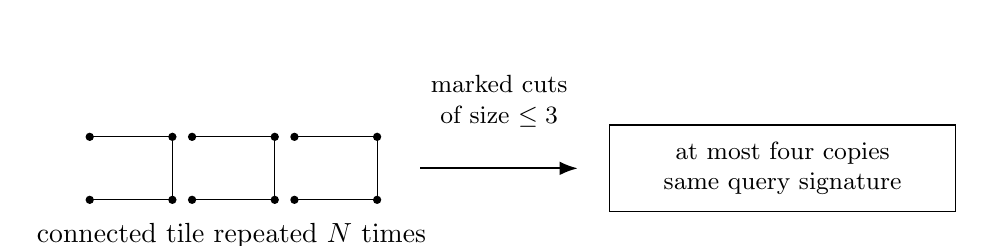
\begin{tikzpicture}[x=1cm,y=1cm,>=Latex]
\foreach \x in {0,1.3,2.6} {
 \draw (\x,0)--(\x+1.05,0);
 \draw (\x,0.8)--(\x+1.05,0.8);
 \draw (\x+1.05,0)--(\x+1.05,0.8);
 \fill (\x,0) circle (1.5pt);\fill (\x,0.8) circle (1.5pt);
 \fill (\x+1.05,0) circle (1.5pt);\fill (\x+1.05,0.8) circle (1.5pt);
}
\node at (1.8,-0.45) {connected tile repeated $N$ times};
\draw[->,thick] (4.2,0.4)--(6.2,0.4);
\node[align=center,font=\small] at (5.2,1.25) {marked cuts\\of size $\le3$};
\draw (6.6,-0.15) rectangle (11.0,0.95);
\node[align=center,font=\small] at (8.8,0.4) {at most four copies\\same query signature};
\end{tikzpicture}
\caption{The reduction is an equivalence for a boundary cut query. It is not an isotopy, a graph isomorphism, or permission to replace a 3-dimensional region by the pictured kernel.}
\end{figure}

\section{Contextual replacement and a width-independent polynomial kernel}
\subsection{Arbitrary external contexts}
An external graph context meets a tile only at its named input and output vertices. It may add edges, connect different tile macros, or impose further identifications among named boundary vertices. Macro interiors and their edge occurrences must be fresh. A \emph{flat repetition descriptor} is an explicitly stored context $H$ together with explicitly stored connected tiles $T_1,\ldots,T_s$ and positive binary exponents $N_1,\ldots,N_s$, where each macro stands for $T_i^{\circ N_i}$. There is no recursively duplicated macro definition in this flat model.

\begin{theorem}[Contextual four-copy kernel]
\label{thm:kernel}
Replace every macro $T_i^{\circ N_i}$ by $T_i^{\circ\min(N_i,4)}$. The resulting graph $G_\star$ and the original graph $G$ have identical clipped marked cut minima, including versions with additional prescribed colors on context vertices. In particular, $G$ has a marked small cut if and only if $G_\star$ does.

If
\[
 Q=|V(H)|+|E(H)|+\sum_i\bigl(|V(T_i)|+|E(T_i)|\bigr)
\]
includes the explicit interface/wiring records, then $G_\star$ has $O(Q)$ vertices and edges. Its size has no exponential dependence on interface width and no numerical dependence on any $N_i$.
\end{theorem}
\begin{proof}
Fix a coloring of the context and all macro boundary vertices. Each macro contributes a minimum local cost for each exact mark set. The full cost is the sum of macro and context costs; its mark set is their union. Theorem~\ref{thm:four} preserves every macro signature, so minimizing over compatible local mark sets and all boundary colorings preserves the full answer. This also proves the assertion with prescribed context colors.

Every macro contributes at most four explicit tile copies. Gluing can only reduce the number of vertices and does not create extra edges beyond the explicit context. The stated size bound follows.
\end{proof}

This is stronger than an algorithm that first constructs a $2^{2w}$ table and then performs fast exponentiation. The proof may use such a table conceptually, but kernel construction only checks tile connectedness and replaces binary exponents by small integers. This is the principal asymptotic improvement of the present work.

\subsection{Cubic validation without expansion}
For the implemented closed serial-chain specialization, cubicality is checked locally. Each private tile vertex must have degree three. At a repeated seam, corresponding output and input degrees must sum to three. The same sum is checked at every inter-block seam and at the final closure. The check treats a loop as degree two and never merges parallel edge occurrences.

\begin{proposition}[Local degree validation]
These conditions are necessary and sufficient for the expanded closed tile chain to be cubic. They remain valid after every four-copy reduction.
\end{proposition}
\begin{proof}
A private vertex belongs to exactly one tile copy. Every other vertex of the closure is the identification of one output port and one input port, with no further port aliasing in this chain model. Its degree is exactly the sum of their degrees. All edge occurrences remain, even when a closure makes an edge into a loop. Reducing a positive repetition count leaves the same private-vertex and seam conditions.
\end{proof}

For an arbitrary external context, an importer must check the corresponding quotient degree sums, not blindly reuse the serial-chain test. The contextual theorem is more general than the delivered assembler; this implementation boundary is deliberate.

\section{A polynomial certificate engine on the finite kernel}
\subsection{Edge-anchored cuts}
For two edge occurrences $e,f$ with disjoint endpoint sets, force both endpoints of $e$ to color zero and both endpoints of $f$ to color one. Let $\lambda(e,f)$ be the resulting minimum cut value.

\begin{proposition}[Two-anchor factorization]
\label{prop:anchors}
For every finite graph,
\[
 \min_{c:F_G(c)=\{0,1\}}q_G(c)
   =\min_{\substack{e,f\in E(G)\\V(e)\cap V(f)=\varnothing}}\lambda(e,f),
\]
where a minimum over no pairs is infinite. It suffices to consider unordered edge pairs, since exchanging the two colors changes neither the cost nor the marked condition.
\end{proposition}
\begin{proof}
Any marked coloring has a monochromatic edge in each color, and these edges have disjoint endpoint sets. They form a feasible anchor pair. Conversely, a coloring respecting an anchor pair has both edge marks. Minimizing in the two directions gives equality. Loops cause no difficulty: the endpoint set of a loop is a singleton and its edge occurrence is a valid mark.
\end{proof}

For each pair, create a source and sink, attach capacity-four arcs from the source to endpoints of $e$ and from endpoints of $f$ to the sink, and replace each non-loop undirected edge by two opposed unit-capacity arcs. Loops are omitted from the flow network but remain eligible anchors. A cut of capacity at most three cannot sever an anchor arc, so it respects the required colors.

Run integral augmenting paths only until the flow reaches four. If no augmenting path remains earlier, residual reachability gives a cut of value at most three. Otherwise a flow of value four excludes every small cut for that anchor pair. At most four augmentations are needed, independently of graph size.

\subsection{Replayable positive and negative evidence}
A negative finite-kernel certificate contains a shore and its cut-edge list. The checker recounts all edges, verifies the cost at most three, and verifies both edge marks. For a positive certificate, every disjoint anchor pair is accompanied by its residual augmentations reaching flow value four. The checker does not search for augmenting paths; it verifies the listed paths, residual capacities, and accumulated flow value. It also checks that no anchor pair is missing.

The threshold-four anchor capacities are intentional. An anchor arc may itself occur in a cut of value four, but this cannot affect the threshold-three predicate. No claim to recover exact minimum cut values above three is made.

\begin{theorem}[Polynomial certified terminal query]
\label{thm:complexity}
Suppose a flat repetition descriptor represents a nonempty cubic graph $G$, and every capped tile is connected. Let $B=\sum_i\bits(N_i)$ and let $Q$ be its explicit tile/context size. Then a marked small cut of $G$ can be found or excluded in polynomial bit time in $Q+B$.

For a cubic $O(Q)$-size kernel, the bounded-flow search takes $O(Q^3)$ elementary graph operations and its positive augmentation certificate has $O(Q^3\log(Q+1))$ bits. The delivered independent dense-capacity replay checker has the conservative bound $O(Q^4)$ elementary operations. Kernel construction and source-bound count manipulation are polynomial in $Q+B$.

When the descriptor is a faithfully embedded spherical pattern on the boundary of a separately certified ball, the same query decides pattern essentiality.
\end{theorem}
\begin{proof}
By Theorem~\ref{thm:kernel}, the numerical multiplicities can be replaced by integers at most four. There are $O(Q)$ vertices and edges in the kernel. Enumerating anchor pairs takes $O(Q^2)$ iterations. A sparse network can be built in $O(Q)$ work for each pair, and at most four breadth-first augmentations each take $O(Q)$ work. This gives the search bound.

There are at most four path records of length $O(Q)$ per pair. Vertex identifiers take $O(\log(Q+1))$ bits, giving the certificate bound. The independent checker deliberately allocates a dense $O(Q^2)$ capacity array for each pair, giving $O(Q^4)$ work; this is a transparent reference choice rather than a claimed optimal replay bound. A sparse checker could improve that factor.

All kernel indices and flow amounts have polynomially bounded bit length. Exponent comparisons, source hashing, and the source witness counts operate on the supplied binary/hexadecimal integers; they do not enumerate their numerical values. The final topological statement is Theorem~\ref{thm:ball} under its geometric hypotheses.
\end{proof}

\section{Lifting a kernel counterexample to the original graph}
\subsection{A succinct original coloring}
\begin{theorem}[Sparse source witnesses]
\label{thm:lift}
Let a four-copy kernel of a flat connected repetition descriptor have a marked cut of cost at most three. A coloring of the original graph with the same cost and both marks can be represented using at most four local coloring runs per capped macro. It has a verification procedure polynomial in the encoded source size, without expansion. For the implemented serial chains, the checker also outputs at most three original cut-edge addresses and two original monochromatic-edge addresses.
\end{theorem}
\begin{proof}
Consider a macro that has been shortened to four copies. Restrict the kernel coloring to those copies. Since the global cut cost is at most three, at least one copy has zero local cost. The tile is connected, so that copy is monochromatic by Lemma~\ref{lem:zero}. Replace this copy by $N_i-3$ identical monochromatic copies, keeping all other three copies. The input and output colors of the repeated run agree. Its cost is zero, and at least one occurrence of its original edge mark remains. Thus the local boundary colors, cost, and exact mark set are preserved. Perform this independently for every capped macro.

A run stores a bit per local tile vertex and a binary repeat count. For verification, check interface-color agreement, including self-agreement inside a repeated run. Count bichromatic edges in each local coloring and multiply by its repeat count. Union the edge marks. These operations use only explicit tile data and binary arithmetic.

Any run containing $a>0$ cut edges can have repeat count at most $\lfloor3/a\rfloor$. Consequently, all cut-edge addresses can be enumerated: there are at most three. A zero-cost run is skipped, however enormous its multiplicity. For each color, record the first local monochromatic edge that supplies its mark. Addresses consist of a macro/block number, a binary copy index, and a local edge index. Their encoded lengths, and the coloring-run data, are polynomial in the original input size.
\end{proof}

For the exceptional single-edge case in the proof of Theorem~\ref{thm:four}, a long coloring was compressed with possibly lower cost. This does not interfere with lifting: lifting starts from a kernel coloring and only duplicates zero-cost copies. It preserves that kernel coloring's actual cost exactly.

\subsection{What the witness does not yet contain}
The output is a certified cut in the \emph{original abstract pattern graph}. Lemma~\ref{lem:forest} certifies cycles on both shores; it does not require the checker to enumerate those potentially long cycles. Theorem~\ref{thm:ball} gives a violating noose when a spherical embedding is supplied. The package does not construct a full embedded disc in the 3-manifold or transport it backward through a hierarchy. Those operations must use the native source charts and pattern provenance.

Likewise, a positive certificate is a proof that the graph has no forbidden small cut. It must never be relabeled as a ball certificate or an unknot certificate. The code's verdicts, \code{LOW_CYCLIC_CUT} and \code{NO_LOW_CYCLIC_CUT}, deliberately preserve that boundary.

\section{Disconnected tiles: an obstruction and a periodic extension}
\subsection{Why connectedness cannot be silently dropped}
Take a width-two tile with edges $\ell_0r_1$ and $\ell_1r_0$, and no others. It is a matching with a swap of its two interfaces. At cost zero, a mixed boundary coloring is swapped by one copy and restored by two copies. Thus the mixed-to-itself, two-mark signature has value zero at even exponents and is not zero at odd exponents. In particular,
\[
 \Sig_3(T^{\circ5})\ne\Sig_3(T^{\circ6}).
\]
The five-copy general bound and the sharper four-copy bound both fail without their connectedness hypothesis. A geometry producer that sees several parallel strands must not call them a connected tile merely because they share a source face or an integer rank interval.

\subsection{A restricted permutation-zero class}
A useful disconnected class still has a controlled law. Suppose every component of $T$ contains exactly one input port and exactly one output port. The resulting matching of components defines a permutation $\pi$ of the $w$ ports. Let $h$ be its order. Additional private vertices and edges inside each connected component are allowed.

\begin{theorem}[Eventual periodicity with permutation zero-cost transport]
\label{thm:period}
Under these hypotheses, for threshold $k$ put
\[
 C=k+(k+1)h.
\]
For every $N\ge C$,
\[
 \Sig_k(T^{\circ N})
 =\Sig_k\bigl(T^{\circ [C+((N-C)\bmod h)]}\bigr).
\]
\end{theorem}
\begin{proof}
A zero-cost copy is constant on each tile component. Its output coloring is the permutation of its input coloring induced by $\pi$. Its mark set is the set of colors appearing on the ports, because every component has an edge. That set is unchanged by the permutation. A run of $\ell>0$ zero-cost copies can therefore be shortened to the unique $\ell'\in\{1,\ldots,h\}$ with $\ell'\equiv\ell\pmod h$, preserving its endpoints and marks.

A coloring of total cost at most $k$ has at most $k$ positive-cost copies, hence at most $k+1$ zero-cost runs. Shortening each nonempty run as above leaves at most $k+(k+1)h=C$ copies, with length congruent to the original modulo $h$. Since $N\ge C>k$, at least one nonempty zero-cost run exists. It can be extended by any multiple of $h$ without changing its endpoints, cost, or marks. Pad to the canonical length $C+((N-C)\bmod h)$.

Conversely, every low-cost coloring at that canonical length has a zero-cost run and can be extended by multiples of $h$ to length $N$. The clipped minima consequently agree.
\end{proof}

This theorem is included as a proved extension, with a small permutation example in the tests. It is not implemented as a production reduction. The order $h$ can itself be large as a function of width, so the theorem must not be called a width-independent polynomial kernel. Arbitrary disconnected tiles can have a more complicated zero-cost relation than a permutation and are outside this statement.

\section{Implementation and proof boundary}
\subsection{Package structure}
The standard-library package is in \code{code/pattern_kernel/}. The immutable tile model, four-copy producer, finite assembly, capped-flow solver, and source-coloring lift are in \code{core.py}. The checker in \code{verify.py} does not invoke kernel production, finite production assembly, or max-flow search. It independently assembles fresh-copy quotient vertices and checks residual augmentations with a dense capacity representation. Basic input types and local degree validation are shared; this is an independent algorithmic replay path, not a formally verified proof assistant development.

The file \code{signatures.py} is an exponential small-instance oracle. It enumerates local colorings and composes the full four-mark table. It is not on the production path. Its explicit eighteen-vertex cap prevents an accidental large local enumeration.

The command-line entry point accepts a closed tile-chain descriptor and writes a JSON certificate. Exponents and copy indices use hexadecimal strings to avoid dependence on language-level decimal digit limits. Integer booleans are rejected where they could masquerade as counts. Explicit expansion is separately capped and is never called on original huge multiplicities. The default finite-assembly cap is 100,000 copies, including calls through \code{solve}; exhaustion declines the query rather than issuing a graph verdict. The mathematical complexity bound concerns the algorithm without this optional implementation cap.

\subsection{Supported and unsupported operations}
The code implements closed serial chains of equal-width tiles with flat positive repetition counts. The contextual theorem supports more general external wiring mathematically, but no general wiring importer is shipped. Only tiles actually shortened need pass connectedness; a small disconnected block may be retained literally.

The implementation validates cubicality and the supplied combinatorial quotient. It does not validate a sphere embedding. For the prism and triangle-expansion examples below, planarity and the spherical interpretation follow from an explicit family construction in this article. On arbitrary user data, a graph verdict remains just a graph verdict until the geometry contract is checked.

The full native \code{fastunknot} regression suite and native knot benchmarks were not run. The source repository was not modified. The proposed integration is an opt-in terminal operator, not a replacement for a complete fallback.

\section{Reproducible evidence}
\subsection{Tests and independent audits}
The retained unit log reports 35 passing tests. These cover input validation, loops and multiple edges, the sharp single-edge example, connected signature stabilization, the disconnected parity counterexample, source lifting, enormous multiplicities, producer-disabled replay, and malformed certificates.

The separate audit uses seed 2026101204 and records the following completed comparisons:
\begin{center}
\begin{tabular}{>{\raggedright\arraybackslash}p{0.69\linewidth}r}
\toprule
Check & Completed\\
\midrule
Connected random tiles, widths one through three & 1,500\\
Full marked signature comparisons, exponents five through eight vs. four & 6,000\\
Random cubic multigraphs vs. exhaustive vertex colorings & 180\\
Spherical simple cubic graphs vs. independently constructed dual criterion & 25\\
\bottomrule
\end{tabular}
\end{center}
The multigraph audit includes loops, parallel edges, and disconnected graphs. The planar audit includes $K_4$, the cube, the dodecahedron, circular ladders, and successive triangle expansions. It reconstructs a planar embedding and dual, then independently checks simplicity and the relevant small vertex-separation condition. The optional oracle dependency was NetworkX 3.6.1; the production package has no dependency on it.

These are exhaustive comparisons \emph{within each sampled finite instance}, not an exhaustive classification of all tiles or cubic graphs. They corroborate the proofs but do not replace them.

\subsection{Large binary examples}
The descriptor for a prism with $2^{16384}+1$ repeated tiles reduces to an eight-vertex, twelve-edge kernel. Its positive JSON proof, including source-bound metadata, occupies 38,174 bytes in the retained formatting. No original vertex or edge list is expanded.

For a negative example, place one triangle-expansion tile between $2^{4096}+7$ ordinary prism tiles and $2^{1024}+9$ ordinary prism tiles. Replacing a cubic vertex by a triangle preserves a spherical cubic embedding. The three edges joining the triangle to the rest of the graph form a marked cut. The kernel has twenty vertices and thirty edges. Its 5,358-byte retained proof lifts to the original descriptor and yields exactly three source edge addresses. The complete source-coloring certificate is verified with binary arithmetic rather than by expanding either long run.

\subsection{Paired performance measurements}
Both timed arms answer the same \emph{boundary graph predicate and replay a certificate}. The explicit arm expands the entire finite prism, runs the bounded-flow certificate engine, and replays its graph certificate. The kernel arm constructs the four-copy reduction, runs the same graph engine, and additionally replays the source reduction. Input parsing, serialization, spherical geometry validation, and knot recognition are outside both timers. Garbage collection is performed before, not inside, each measurement.

Each completed case has one warmup and five paired rounds, with arm order shuffled using a fixed seed. The reported ratio is the median of the five within-round explicit/kernel ratios; it need not equal the ratio of the two separately reported medians. The machine and interpreter strings, all rounds, and a control are retained in \code{experiments/benchmark.json}.

\begin{center}
\begin{tabular}{rrrr}
\toprule
Copies & Explicit median (ms) & Kernel median (ms) & Paired ratio\\
\midrule
1 & 0.098 & 0.238 & 0.407\\
3 & 0.125 & 0.281 & 0.431\\
4 & 1.389 & 1.528 & 0.919\\
8 & 9.904 & 1.552 & 6.371\\
16 & 69.882 & 1.616 & 43.090\\
32 & 545.921 & 1.551 & 351.250\\
\bottomrule
\end{tabular}
\end{center}


The identical-explicit A/A control at sixteen copies has median ratio 0.974. The one-, three-, and four-copy cases expose real overhead: there is little or nothing to reduce. At thirty-two copies, the complete graph-query/replay ratio is approximately $351.25$. This is an advantage over the shipped explicit reference path, not a comparison with the best known cubic-connectivity implementation and not an end-to-end knot-recognition speedup.

The large binary kernel-only medians for exponents $2^{128}+1$, $2^{1024}+1$, $2^{4096}+1$, and $2^{16384}+1$ were respectively 1.589, 1.492, 1.617, and 1.949 milliseconds in the retained run. Those examples have the same constant-size graph kernel; their input arithmetic and source binding still depend on encoded bit length.

An earlier benchmark driver attempted to include sixty-four copies but hit its sixty-second process limit before writing the final result file. Its partial console ratios are not used in the published table. The exclusion and driver hash are recorded in \code{experiments/benchmark_timeout.json}. The final table contains only the separately completed rerun.

\section{Repository integration and a roadmap clarification}
\subsection{A concrete adapter contract}
A future geometric adapter should produce a source-bound descriptor with all of the following information: the actual embedded boundary graph, the ordered tile interfaces, a proof that capped tiles are connected, edge ownership and source addresses, and a certificate that the relevant ambient terminal component is a ball. The graph operator then produces either a four-flow exclusion certificate or a lifted original graph cut.

The existing source-parallelity packet is a natural place to seek these tiles because it retains interfaces, fibre bits, and source charts. However, the existence of an $O(T)$ inherited core does not prove that every transported boundary pattern has a short flat connected-repetition descriptor. A port mask also does not encode cyclic boundary order or all subsequent pattern attachments. The adapter must retain those facts rather than infer them from Euler characteristic or a component count.

In particular, no automatic identification is made here between a parallelity component and a connected graph tile. Several strands in one product family can be a disconnected graph tile; Section~8 shows why that distinction changes the algebra.

\subsection{A documentation update, not a claimed mathematical correction}
At the inspected checkpoint, the root README's compressed-geometry paragraph still points primarily to raw-cut and cut-boundary construction, while the source-parallelity article already describes a bounded \emph{inherited} complementary core. The proposed README insertion distinguishes this implemented source-core result from the still-missing \emph{admissible patterned} hierarchy structure. It does not delete the latter open obligation or claim a general complexity theorem \cite{repo-readme,repo-parallelity}.

No concrete false theorem in the inspected parallelity article is established by this work. Its distinctions among raw cuts, source parallelity, source provenance, and later admissibility are retained. The supplied integration note therefore labels the README change as a roadmap clarification, not as a correction to a proved geometric result.

\subsection{Safe operational behavior}
The recommended interface is a terminal graph query with an explicit unsupported outcome when a large disconnected tile would need capping. Unsupported compression must not become a positive essentiality answer. Resource exhaustion must remain inconclusive. The existing complete recognizer should remain available without altering its soundness contract.

For positive results, bind the source and all capped exponents to the proof, verify the kernel reconstruction, and require every anchor pair. For negative results, independently verify the original-source coloring, not merely the reduced graph's cut. For a topological consequence, additionally validate the sphere and ball hypotheses. The code intentionally contains no convenience flag such as \code{assume_ball=True}.

\section{Implications for the quasi-polynomial objective}
The result removes a particular source of exponential work: expanding a binary multiplicity before a terminal essentiality test. It does so with a stronger parameter statement than a bounded-width dynamic program. Under a flat connected-repetition description, neither a logarithmic width hypothesis nor a small expanded graph is required.

\begin{corollary}[Conditional hierarchy cost substitution]
Suppose a complete, geometrically verified recognition procedure makes $H(n)$ terminal queries on faithful flat connected-repetition descriptors of encoded sizes at most $S(n)$, and spends $A(n)$ on all other operations, including descriptor production and transport of certificates. Replacing explicit terminal expansion by the present certified operator gives total time
\[
 A(n)+H(n)\poly(S(n)).
\]
Consequently, if $A(n)$, $H(n)$, and $S(n)$ are all bounded by $2^{(\log n)^{O(1)}}$, the resulting complete procedure is quasi-polynomial.
\end{corollary}
\begin{proof}
Apply Theorem~\ref{thm:complexity} to each descriptor and sum the costs. Products and fixed powers of quasi-polynomial functions are quasi-polynomial.
\end{proof}

The hypotheses are not proved here for arbitrary knot diagrams. In particular, we do not prove a short grammar producer for every transported pattern, a bound for every hierarchy reset and repair, or a global hierarchy depth/discovery bound. The theorem should be used to replace one cost term in an eventual end-to-end accounting, not to skip the accounting.

The most direct experimental next step is not another generic random knot corpus. It is to instrument the source-parallelity/pattern-transport boundary, record candidate tile components and interfaces, and measure how often connected flat repetitions actually occur. That evidence would test whether the proved kernel removes a dominant native cost.

\section{Further research questions}
\begin{enumerate}[leftmargin=*,itemsep=0.7em]
\item \textbf{A faithful producer from source charts.} Can the source-parallelity and cut-boundary records construct a flat connected-repetition descriptor for transported patterns in polynomial encoded time? Which local type transitions force nested rather than flat reuse? A useful first theorem would identify a nontrivial family of normal cuts where the producer is complete.
\item \textbf{General disconnected zero-cost relations.} Theorem~\ref{thm:period} handles a permutation relation. Can zero-cost relations with component merges and splits be decomposed into a polynomial-size transient part and controlled periodic components? Any such theorem must account for the mixed-color parity example.
\item \textbf{Threshold-preserving marked sparsifiers.} Connectivity-threshold mimicking networks preserve terminal cut values \cite{mimicking2020}. Can they be augmented to preserve the two monochromatic-edge witnesses without exponential interface state? Ordinary cut preservation alone does not record those witnesses.
\item \textbf{More efficient positive proof replay.} Replace the reference dense capacity checker by a carefully bounded sparse or shared-flow checker. Can many anchor pairs reuse a certificate without losing independent coverage verification? The production decision bound is already cubic in kernel size, while the deliberately simple checker is quartic.
\item \textbf{A compressed geometric noose.} Starting from the at most three source edge addresses and the succinct coloring, construct a noose in the native embedded pattern with a compressed isotopy/provenance record. Then transport the corresponding disc through the hierarchy without expanding a large repeated region.
\item \textbf{Multiple boundary components and vertex-free loops.} Extend the importer to transport an entire terminal pattern inventory, including vertex-free circles and certified ball ownership. Repeated graph components must be distinguished from repeated components of the 3-manifold.
\item \textbf{Optimal cutoffs for other thresholds and marks.} The general $k+2$ bound is not asserted to be optimal for every $k$. Determine exact stabilization thresholds for richer local witness monoids, and determine which integral edge-weight assumptions permit the four-copy argument unchanged.
\item \textbf{End-to-end hierarchy accounting.} Establish source-complete grammar size, ball certification, repair/reset work, and the number of terminal queries together. Only their combined bound can support an unrestricted quasi-polynomial theorem for the recognizer.
\end{enumerate}

\section{Conclusion}
Connected repetition has substantially more structure than an arbitrary compressed graph. At threshold three, its full marked boundary-cut signature stabilizes after four copies, with a sharp constant and no interface-width dependence. This yields a polynomial-size terminal query kernel and source-addressable counterexamples even for enormous binary multiplicities.

The geometric and algorithmic boundaries remain explicit. A four-copy kernel is not a replacement 3-manifold. A graph cut certificate is not a ball certificate. The supplied implementation is a tested, separately replayed terminal operator, not an unrestricted quasi-polynomial recognizer. Its potential contribution to that objective is concrete: once faithful connected repetition is available at the pattern interface, numerical multiplicity no longer drives the terminal query cost.

\appendix
\section{Reproduction and file inventory}
From the package root, run:
\begin{verbatim}
PYTHONPATH=code python -m unittest discover -s tests -v
PYTHONPATH=code python experiments/audit.py
PYTHONPATH=code python experiments/benchmark.py
PYTHONPATH=code python -m pattern_kernel \
  examples/huge_prism.json --output replayed-proof.json
cd article && sh build.sh
\end{verbatim}
The test suite and production code need Python 3.10 or later and its standard library. The planar-dual audit additionally needs NetworkX; the recorded version is 3.6.1. The tested interpreter was CPython 3.13.5 on Linux x86-64. The article builds with pdf\LaTeX. Benchmarks are machine-specific and should be rerun rather than treated as universal constants.

\begin{longtable}{>{\raggedright\arraybackslash}p{0.38\linewidth}>{\raggedright\arraybackslash}p{0.56\linewidth}}
\toprule
Path & Purpose\\\midrule\endhead
\code{article/four_copy_patterns.tex} & Full article and proofs.\\
\code{article/four_copy_patterns.pdf} & Compiled, visually inspected article.\\
\code{code/pattern_kernel/core.py} & Kernel producer and finite certificate engine.\\
\code{code/pattern_kernel/verify.py} & Search-free independent replay and original-source witness checks.\\
\code{code/pattern_kernel/signatures.py} & Exponential independent oracle, with a strict local-size cap.\\
\code{tests/test_kernel.py} & Maintained standalone test suite.\\
\code{experiments/audit.json} & Completed audit counts, environment, and large-case sizes.\\
\code{experiments/benchmark.json} & Raw paired rounds, medians, A/A control, and binary cases.\\
\code{experiments/benchmark_timeout.json} & Excluded incomplete larger benchmark attempt.\\
\code{examples/} & Source descriptors, replayable proofs, and sparse edge addresses.\\
\code{integration/INTEGRATION.md} & Native adapter contract and outstanding obligations.\\
\code{integration/README-roadmap.patch} & Proposed source-roadmap insertion, not applied.\\
\code{source_manifest.json} & Inspected repository paths and content pins.\\
\code{SHA256SUMS} & Hashes of distributed artifacts.\\
\bottomrule
\end{longtable}

\section{Proof and implementation status ledger}
\begin{longtable}{>{\raggedright\arraybackslash}p{0.40\linewidth}>{\raggedright\arraybackslash}p{0.54\linewidth}}
\toprule
Item & Status\\\midrule\endhead
Primal marked-cut criterion & Proved here, as a reformulation of the terminal condition; classical cyclic-cut ingredients are acknowledged.\\
General connected $k+2$ cutoff & Proved; small thresholds independently tested.\\
Sharp four-copy threshold-three theorem & Proved; 6,000 independent full-signature comparisons retained.\\
Flat contextual kernel & Proved; closed serial-chain specialization implemented.\\
Polynomial graph certificate engine & Implemented and independently replayed; reference checker has conservative quartic cost.\\
Original-source sparse witnesses & Implemented; enormous binary positive and negative cases retained.\\
Permutation-zero eventual periodicity & Proved; a swap example tested; production reduction not implemented.\\
General embedded-pattern importer & Not implemented or proved complete.\\
Native geometry-to-tile integration & Not run.\\
Native full regression and knot benchmarks & Not run.\\
Unrestricted quasi-polynomial recognizer & Not established by this work.\\
External novelty/priority certification & Not established; targeted literature comparison only.\\
\bottomrule
\end{longtable}

\begin{thebibliography}{9}
\bibitem{lackenby2026}
M.~Lackenby, \emph{Incompressible surfaces, hierarchies and unknot recognition}, arXiv:2607.23350v1, 25 July 2026. In particular, the ball-pattern criterion and the hierarchy running-time discussion.\newline
\url{https://arxiv.org/html/2607.23350v1}

\bibitem{cyclic2004}
Z.~Dvo\v r\'ak, J.~K\'ara, D.~Kr\'al', and O.~Pangr\'ac, \emph{An Algorithm for Cyclic Edge Connectivity of Cubic Graphs}, Algorithm Theory---SWAT 2004, Lecture Notes in Computer Science 3111, pp.~236--247. DOI: 10.1007/978-3-540-27810-8\_21.\newline
\url{https://link.springer.com/chapter/10.1007/978-3-540-27810-8_21}

\bibitem{mimicking2020}
P.~Chalermsook, S.~Das, B.~Laekhanukit, Y.~Kook, Y.~P.~Liu, R.~Peng, M.~Sellke, and D.~Vaz, \emph{Vertex Sparsification for Edge Connectivity}, arXiv:2007.07862, 2020.\newline
\url{https://arxiv.org/abs/2007.07862}

\bibitem{repo-parallelity}
\emph{ProveIt: Source parallelity in all handle dimensions and a bounded inherited core}, \code{Topology/UnknotRecognition/synthesis/parallelity.tex}, inspected at commit \code{ed166080d7db14dd7a91d07788996f02947dd92a}.\newline
\url{https://github.com/VladimirReshetnikov/ProveIt/blob/ed166080d7db14dd7a91d07788996f02947dd92a/Topology/UnknotRecognition/synthesis/parallelity.tex}

\bibitem{repo-readme}
\emph{ProveIt: UnknotRecognition README}, \code{Topology/UnknotRecognition/README.md}, same inspected commit.\newline
\url{https://github.com/VladimirReshetnikov/ProveIt/blob/ed166080d7db14dd7a91d07788996f02947dd92a/Topology/UnknotRecognition/README.md}
\end{thebibliography}
\end{document}
